\documentclass[a4paper,12pt]{article}
\usepackage{datetime}
\usepackage{geometry}
\geometry{a4paper}

\usepackage{graphicx}
\usepackage{svg}
\usepackage{amssymb}
\usepackage{epstopdf}
\usepackage{endnotes}
\let\footnote=\endnote
\setlength\parindent{0pt}
\setlength{\parskip}{6pt}
\DeclareGraphicsRule{.tif}{png}{.png}{`convert #1 `dirname #1`/`basename #1 .tif`.png}

\newcommand{\proj}{AnonEvote}

\title{\proj{}\\A Project on Blockchain Evoting\\Functional Specification}
\author{Michael Wall\\13522003}
\date{\today}

\begin{document}
\maketitle

\vspace{4cm}
\begin{center}\begin{tabular}{|l|l|}
	\hline
	\textbf{Version} & \textbf{Comments} \\ \hline
	0.1 & Initial Draft.\\ \hline
\end{tabular}\end{center}

\newpage
\section{Introduction}
This document describes an implementation of an electronic voting system which utilises a blockchain\footnote{A blockchain is a distributed database which maintains a growing ledger of records called blocks. Each block is timestamped and linked to the previous block to create the chain. The data in a block cannot be altered without breaking the chain} database. The system is used to allow a user to electronically cast a vote in an anonymous, verifiable and tamper-proof manner. Voters fill out a ballot which is ecnrypted to form a transaction. This is then broadcast over a peer-to-peer network. The final vote can be counted and verified by any user, but no users' ballots can be traced back to a voter.

The need for this system arises from the lack of a secure, trustless, tamper-proof and anonymous electronic voting system. Paper ballots are slower, and more expensive to conduct (work hours to organise polling stations, tallying votes, re-counts of votes, multiple voting options, errors filling out a ballot, etc). The \proj{} system aims to tackle some of these issues.

\begin{description}

    \item[Peer-to-peer network (P2P)]
        A peer-to-peer network is a distributed networking architecture in which peer nodes are equal and can act as both a "client" and a "server" for other nodes on the network. It eliminates the need for a centralized server. We will refer to the peer-to-peer network as a P2P network from here on.

	\item[Blockchain]
		The blockchain is the distributed database which maintains the \textit{ledger} of \textit{ballots}. It is broadcast to all participants in the system via the P2P network. Each client will maintain an up-to-date version of the \textit{ledger} to the best of their knowledge. The requirements for the blockchain are described further in section \S\ref{subsec:blockchain} on page \pageref{subsec:blockchain}.

	\item[Ledger]
		The \textit{ledger} is a growing record of all \textit{ballots} which have been cast. The ledger is comprised of a series of \textit{blocks}, each block referring to the previous block to form a chain.

    \item[Block]
        Each \textit{block} contains a set number of \{transactions}. Transactions are publicly viewable, but their contents are secured using cryptographic encryption.

	\item[Transaction]
		Each transaction in a \textit{block} contains a single \textit{ballot}, which has been encrypted to provide anonymity and to prevent tampering.

    \item[Ballot]
        A \textit{ballot} is the form which a voter fills out to cast their \{vote}.

\end{description}

\section{General Description}
\subsection{Product/System Functions}
The \proj{} system is designed to enable electronic voting to be carried out securely, tamper-proof and anonymously. A user of the system will cast a vote electronically through some user interface. The user's vote is then encrypted to form a \textit{secured vote}. The user can verify that their vote is what they intended by decrypting it. This will spoil the ballot, but after repeated casting and decrypting the user can be sure that their vote is accurate. When the user is happy with their ballot, it is then broadcast to all of the client's peers to be verified. The verification of the transaction requires a proof of work to be a valid block. This proof of work entails some computationally expensive task. When the proof of work is complete, the block is then broadcast to a client's peers. If there is disagreement between a new block, consensus is used to select the correct version which is then broadcast to all peers.

To verify their vote, a user can look at the blockchain and verify that their receipt exists on the chain. Homomorphic encryption of votes allows them to be tallied without decrypting individual votes. Any user will be able to perform the computation to tally the votes.

\subsection{User Characteristics}
A user will be any eligible voter. The users are not expected to require any prior knowledge of blockchains, cryptography or other technical concepts described in this document. Because different users may have different user needs or certain levels of ability, the system must be accessible. As a graphical user interface is not a major priority for the system, this challenge will not be addressed to any major extent. The system will be used by text inputs, similar to a command line program, on top of which a UI can be built at a later date.

A user should be able to input a vote, and verify their selection. Once the user has made their selections, they should be able to validate the encryption of their vote as many times as they see sufficient. Once the user is happy that the system is registering their intended vote, the user should then be able to cast their vote to the network to have the transaction verified and added to the ledger. The user should also receive a digital receipt of their transaction so that they can verify their vote at a later date. The user should also be able to perform the required computation to tally the votes should they wish to do so.

\subsection{Operational Scenarios}
\subsubsection{Main}
The main scenario in which the system is intended to be used is any large scale elections, referendums or other votes in which a large body of people will participate in. These votes are required to provide anonymity to voters, tamper-proof security, easy tallying and re-counting of ballots, and a trustless\footnote{A trustless environment is one in which no one individual or group requires to be trusted to ensure the integrity of the system. For example, a bank is not trustless, as you must trust the bank to keep its record of your account accurate and free from tampering.} environment.

\subsection{User stories}
\subsubsection{User casts a vote which is valid}
A user selects candidate A on their electronic ballot. They verify that their selection was correctly registered and cast the vote. Their vote is then verified by peers on the network and added to the ledger.

\subsubsection{User ranks 3 out of 5 options on their ballot}
A user selects candidate options A, D and E on their ballot. They choose not to rank the last two options B or C. Their vote is verified, and added to the ledger.

\subsubsection{User selects no options on their ballot}
A user chooses not to select an option on their ballot. This is represented as selecting a "None of the above" option for the purposes of the vote.

\subsubsection{User spoils their ballot by selecting wrong options}
The user selects both candidate A and B on their electronic ballot. The system will not allow an incorrect selection such as this, and alerts the user to the error. The user then starts the process from the start.

\subsection{Constraints}
\label{ssec:constraints}
A voting system in general needs a few things to make it fair. A prime factor of a successful voting system is that a voter should not be able to sell their vote. For this requirement to be met, a user should have no way of proving what way they filled out their ballot to the outside world. This also means that the ballot itself should have no way of identifying who filled it out.

Ballots should also not be tamperable. This is why some voting systems use pencil instead of pens, to ensure that no erasing ink could be used to invalidate a voter's ballot.

Different voting systems\footnote{A voting system consists of the set of rules which must be followed for a vote to be valid, and defines how otes are cast, counted and aggregated to yield the final result. Examples include a plurality, majority representation and many other variations.} also have different requirements.

In the simplest case a voting system in which a voter selects a single option from two or more choices, and the option with the most votes wins. Other systems are more complicated and require more complicated comutation to achieve a result.

Such systems include weighted voting systems, proportional, semi-proportional, rated and multiple winner systems. Such systems pose challenges as the votes may not be very easily calculated as with a simple tally.

Some voting systems also require the polling statistics to be kept a secret until the end of the vote. This could prevent early predictions from causing a swing in the vote due to people believing that a particular candidate has already won.

Each voting system would require its own rules to specified for the vote to be successful. For this reason the \proj{} system will focus on two systems as a proof of concept, with the ability to add more systems. The two systems will be \textit{Proportional Reprisentation with a Single Transferable Vote}\footnote{The PR-STV system is used in Ireland.} and \textit{Party List Proportional Representation}\footnote{The Party List PR system is used in 85 countries}.

\section{Functional Requirements}

\subsection{Secure Votes}
\label{subsec:securevote}

\subsubsection{User can access the system}
\begin{description}
	\item[Description]
		A user should be able to securely access the system and be verified to cast their vote. The no user should be able to masquerade as another user to cast their vote.
	\item[Criticality]
		Low
	\item[Technical issues]
		It is a challenge to authenticate a single user, as the method of registering for the system must ensure that each citizen can only have one account, and that no other citizen can use another's account. It is expected that this authentication of users will be managed by a third party who wishes to implement this system.
	\item[Dependencies on other requirements]
		None.
\end{description}

\subsubsection{User can make selections on their ballot}
\begin{description}
	\item[Description]
		A user should be able to input the appropriate options on their ballot, including multiple selections, scorings, abstaining from selections etc.
	\item[Criticality]
		High
	\item[Technical issues]
		A certain type of vote may require text input, in which case the user could enter an error or mispelling into the system.
	\item[Dependencies on other requirements]
		This is dependent on \ref{sssec:vote-sys-rep}.
\end{description}

\subsubsection{User can verify their ballot is as intended}
\begin{description}
	\item[Description]
		A user should be able to verify that their input ballot is encrypted as intended. This may invlove decrypting their transaction before it is broadcast to the network in order to verify that it represents their intended ballot. This will invalidate this particular encryption of the ballot. The user should be able to perform this a number of times until they are sufficiently sure that the system is correctly representing their vote.
	\item[Criticality]
		High
	\item[Technical issues]
		It may be an issue that once a transaction is decrypted, the network should know that it is invalid and so not accept it into the ledger.
	\item[Dependencies on other requirements]
		This is dependent on \ref{sssec:ballot-enc-trans}.
\end{description}

\subsubsection{A user cannot reveal the contents of their ballot to the outside world}
\begin{description}
	\item[Description]
		In order to satisfy the constraints described in \ref{ssec:constraints}, a user should not be able to reveal what way they filled out their ballot to the outside world.
	\item[Criticality]
		High
	\item[Technical issues]
		The votes must be countable without a user being able to identify the vote as their own.
	\item[Dependencies on other requirements]
		This is dependent on \ref{sssec:ballot-enc-trans}.
\end{description}

\subsubsection{The ballot can be encrypted and formed into a transaction}
\label{sssec:ballot-enc-trans}
\begin{description}
	\item[Description]
		A ballot should be represented in some agreed format, and encrypted so as the contents of the ballot are protected, and that no user can have their vote identified.
	\item[Criticality]
		High
	\item[Technical issues]
		It is a huge issue to ensure that a user cannot link their vote to their identity, as this enables the sale of votes. The result of the vote should be calculatable, while also not revealing information about the voter.
	\item[Dependencies on other requirements]
		This is dependent on \ref{sssec:vote-sys-calc} and \ref{sssec:vote-sys-view}.
\end{description}

\subsection{Blockchain}
\label{subsec:blockchain}

\subsubsection{A client node can broadcast to its peers}
\label{sssec:blk-comms}
\begin{description}
	\item[Description]
		A peer-to-peer network will be required to enable a node to broadcast transactions, blocks and other necessary information to other nodes involved in maintaining the system.
	\item[Criticality]
		High
	\item[Technical issues]
		Node discovery on the peer-to-peer network may be problematic without the use of a peer discovery server or installed lists of peers to begin seeding the network.
	\item[Dependencies on other requirements]
		None.
\end{description}

\subsubsection{A node can verify a transaction and create a block}
\begin{description}
	\item[Description]
		A node should perform some cryptographic operation which is computationally expensive, like a proof of work, in order to verify a transaction and create a block for the network.
	\item[Criticality]
		High
	\item[Technical issues]
		Selecting a proof of work of sufficient difficulty without being too expensive. If a transaction can be verified instantaneously, it becomes easier to hack the system. If it takes too long to verify, then the user could have to wait an inconvenient amount of time before their vote is successfuly added to the system.
	\item[Dependencies on other requirements]
		None.
\end{description}

\subsubsection{Nodes can add new blocks to the chain using a consensus}
\begin{description}
	\item[Description]
		Nodes should be able to agree on the correct version of the voting history using consensus. This would mean to hack the system an attacker would need to be in control of 51\% of the nodes in the network. This is not feasible in a large scaling system.
	\item[Criticality]
		High
	\item[Technical issues]
		This may be a generally difficult task to complete across a network of peers where fully operational communications are not guaranteed, and not all peers are guaranteed to be connected at all times.
	\item[Dependencies on other requirements]
		This is dependent on \ref{sssec:blk-comms}.
\end{description}

\subsection{Voting System}

\subsubsection{A particular voting system can be implemented}
\label{sssec:vote-sys-rep}
\begin{description}
	\item[Description]
		Ideally, the style of voting sytem used should be independent from the blockchain implementation, meaning the system can be used in different regions which require different rules and regulations. However, the system will be required to work on at least one system as a proof of concept.
	\item[Criticality]
		High
	\item[Technical issues]
		If homomorphic encryption is to be used to tally votes, this may not work in some voting systems which are not a simple count, but have weighting towards votes and different criteria for an outcome to be determined.
	\item[Dependencies on other requirements]
		This is dependent on \ref{sssec:vote-sys-calc} and \ref{sssec:ballot-enc-trans}.
\end{description}

\subsubsection{The ledger can be processed to obtain a vote's result}
\label{sssec:vote-sys-calc}
\begin{description}
	\item[Description]
		The sytem should be implemented in such a way as to allow the result of the vote to be calculated without compromising voter identities or linking votes to voters.
	\item[Criticality]
		High
	\item[Technical issues]
		This faces very similar issues as mentioned in \ref{sssec:vote-sys-rep}.
	\item[Dependencies on other requirements]
		This is dependent on \ref{sssec:vote-sys-rep} and \ref{sssec:ballot-enc-trans}.
\end{description}

\subsubsection{A user can see their vote in the ledger}
\label{sssec:vote-sys-view}
\begin{description}
	\item[Description]
		A user should be able to see that their ballot has been added to the ledger correctly. They should be able to do this without identifying it as their vote and without revealing the contents of the vote.
	\item[Criticality]
		Medium
	\item[Technical issues]
		A user should not be able to identify the contents of their ballot so as to avoid the selling of votes.
	\item[Dependencies on other requirements]
		None.
\end{description}

\section{System Architecture}
Please see Figure \ref{fig:system-architecture} on page \pageref{fig:system-architecture} for the diagram. The system architecture consists of a network of nodes, all of which run the client software. Nodes are connected to form a peer-to-peer network.

\begin{figure}[ht]
\centering
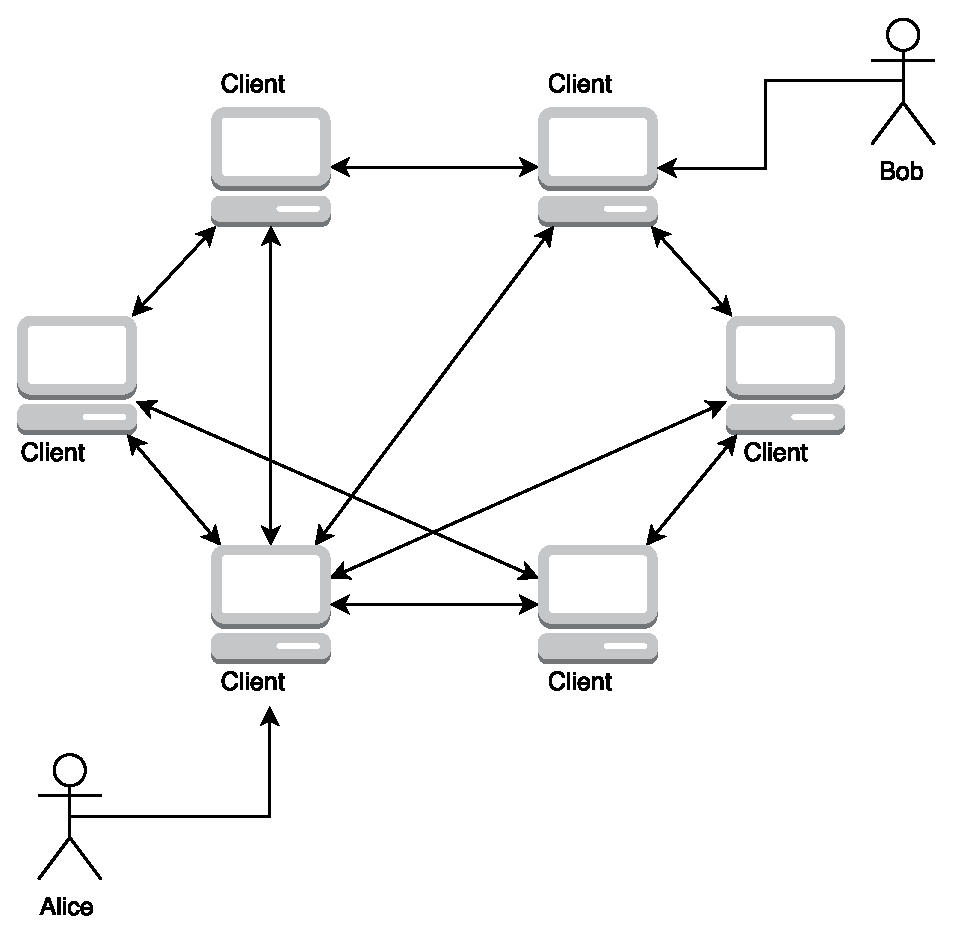
\includegraphics[width=\textwidth]{SystemArchitecture.eps}
\caption{The system consists of a peer to peer network of nodes, all of which are running the client software. The user interacts with the system through a node running the client software.}
\label{fig:system-architecture}
\end{figure}

\section{High Level Design}
Please see Figure \ref{fig:high-level-design} on page \pageref{fig:high-level-design} for the diagram. A user will interact with the system to perform completion of their ballot. The client node will independently carry out peer discovery. It is not required that a node communicate with specific peers on the network. A node will perform encryption of a ballot and broadcasting of transactions for its user. It will also perform transaction verification, consensus agreements, and chain updating in collaboration with other peers on the network. Any node can perform these functions if they are running the client software.

\begin{figure}[ht]
\centering
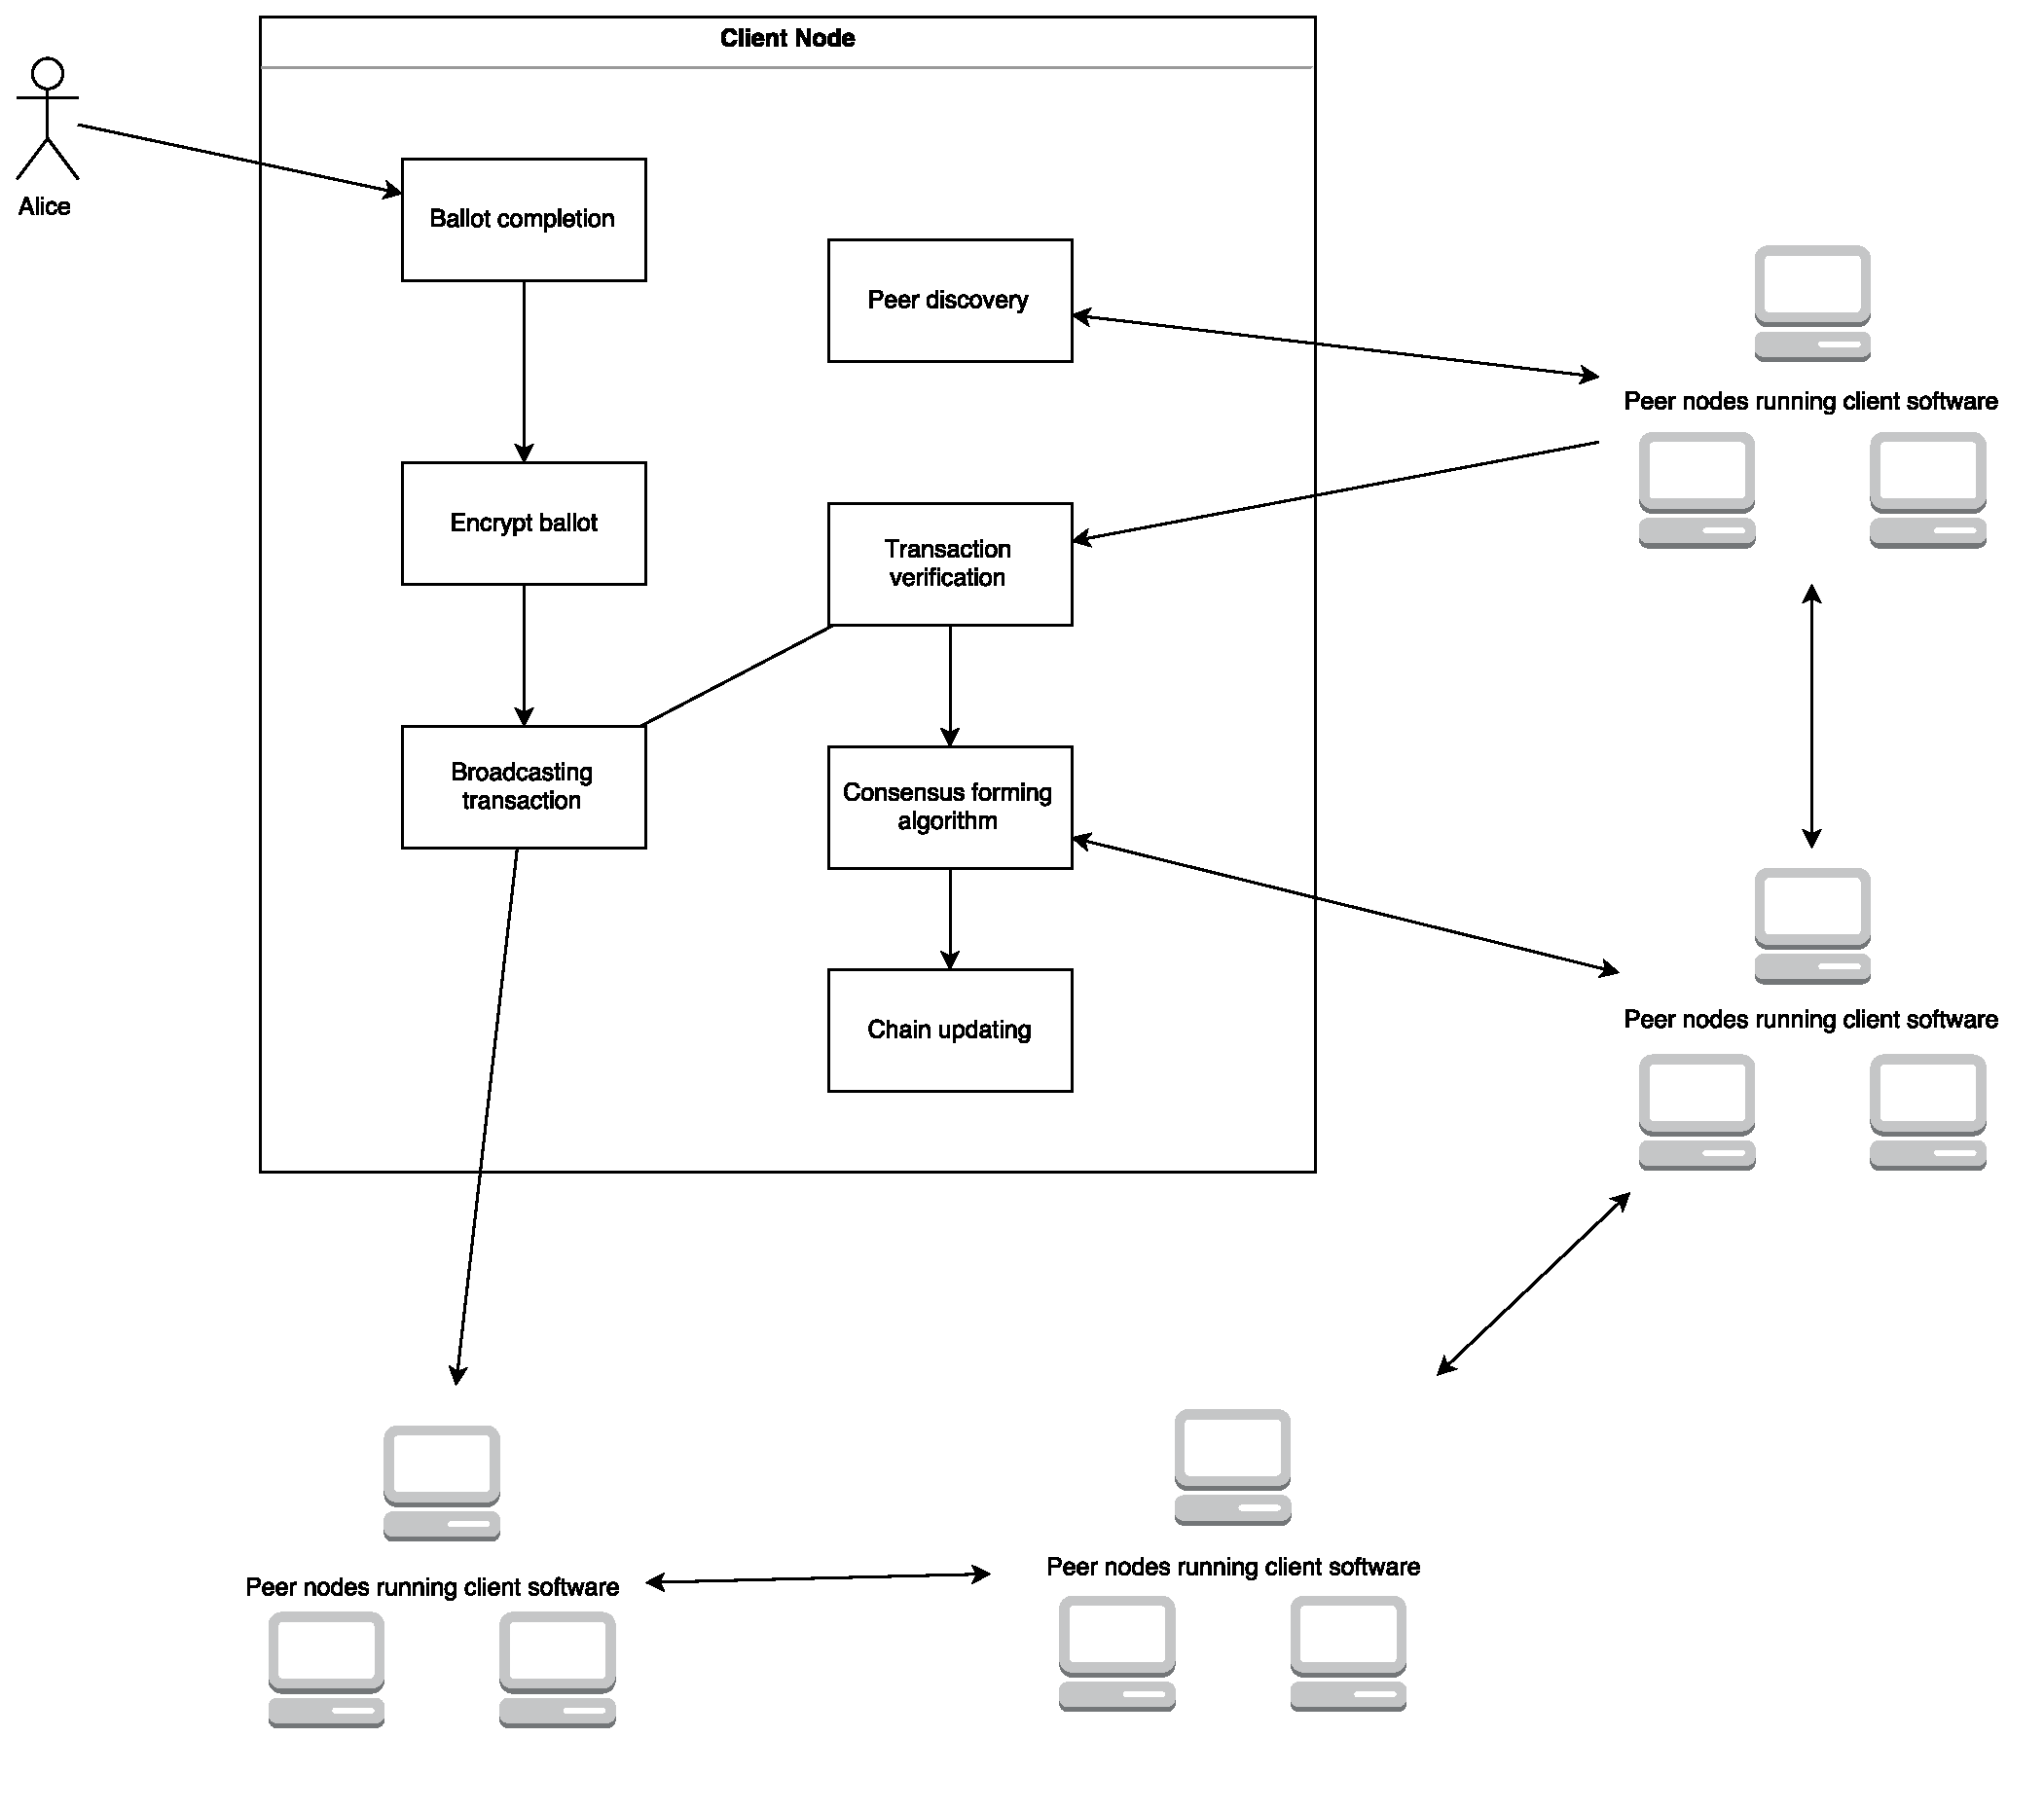
\includegraphics[width=\textwidth]{HighLevelDesign.eps}
\caption{This diagram shows the high level design of the system. The image depicts the functions which a client node must perform. A user of the system will interact with ballot completion. A node can communicate with any of its peers for successful operation.}
\label{fig:high-level-design}
\end{figure}

\section{Development schedule}
My project will not consist of a traditional schedule which has a large block of time for research, then development and then testing or polishing of the project. I will instead be using an agile approach for development.

I will be working with a sprint duration of two weeks, enabling sufficient time for research and development of selected tasks, while also ensuring that any necessary feedback can be provided between sprints. Any issues that arise during a sprint can be dealt with before progressing further with the project.

Tasks for any given sprint will be selected from the project backlog at the beginning of the sprint. Any new issues will be added to the backlog as the project progresses. Any tasks which require grooming will be expanded into more specific sub tasks which are suitable for development in a sprint.

I will be using a private repository on GitHub to manage my code, and will push changes to my GitLab repository frequently. I will use \textit{Waffle.io} to manage the project backlog and to track issues. This system will be integrated with the GitHub repository. I will use a Travis server to perform continuous integration testing where applicable.

\newpage
\theendnotes
\end{document}
